\documentclass[paper=letter,11pt]{scrartcl}

\KOMAoptions{headinclude=true, footinclude=false}
\KOMAoptions{DIV=14, BCOR=5mm}
\KOMAoptions{numbers=noendperiod}
\KOMAoptions{parskip=half}
\addtokomafont{disposition}{\rmfamily}
\addtokomafont{part}{\LARGE}
\addtokomafont{descriptionlabel}{\rmfamily}
%\setkomafont{pageheadfoot}{\normalsize\sffamily}
\setkomafont{pagehead}{\normalsize\rmfamily}
%\setkomafont{publishers}{\normalsize\rmfamily}
\setkomafont{caption}{\normalfont\small}
\setcapindent{0pt}
\deffootnote[1em]{1em}{1em}{\textsuperscript{\thefootnotemark}\ }


\usepackage{amsmath}
\usepackage[varg]{txfonts}
\usepackage[T1]{fontenc}
\usepackage{graphicx}
\usepackage{xcolor}
\usepackage[american]{babel}
% hyperref is needed in many places, so include it here
\usepackage{hyperref}

\usepackage{xspace}
\usepackage{multirow}
\usepackage{float}


\usepackage{braket}
\usepackage{bbm}
\usepackage{relsize}
\usepackage{tcolorbox}

\def\ketY{\ensuremath{\ket {\Psi}}}
\def\iGeV{\ensuremath{\textrm{GeV}^{-1}}}
%\def\mp{\ensuremath{m_{\textrm{proton}}}}
\def\rp{\ensuremath{r_{\textrm{proton}}}}
\def\me{\ensuremath{m_{\textrm{electron}}}}
\def\aG{\ensuremath{\alpha_G}}
\def\rAtom{\ensuremath{r_{\textrm{atom}}}}
\def\rNucl{\ensuremath{r_{\textrm{nucleus}}}}
\def\GN{\ensuremath{\textrm{G}_\textrm{N}}}
\def\ketX{\ensuremath{\ket{\vec{x}}}}
\def\ve{\ensuremath{\vec{\epsilon}}}


\def\ABCDMatrix{\ensuremath{\begin{pmatrix} A &  B  \\ C  & D \end{pmatrix}}}
\def\xyprime{\ensuremath{\begin{pmatrix} x' \\ y' \end{pmatrix}}}
\def\xyprimeT{\ensuremath{\begin{pmatrix} x' &  y' \end{pmatrix}}}
\def\xy{\ensuremath{\begin{pmatrix} x \\ y \end{pmatrix}}}
\def\xyT{\ensuremath{\begin{pmatrix} x & y \end{pmatrix}}}

\def\IMatrix{\ensuremath{\begin{pmatrix} 0 &  1  \\ -1  & 0 \end{pmatrix}}}
\def\IBoostMatrix{\ensuremath{\begin{pmatrix} 0 &  1  \\ 1  & 0 \end{pmatrix}}}
\def\JThree{\ensuremath{\begin{pmatrix}    0 & -i & 0  \\ i & 0  & 0 \\ 0 & 0 & 0 \end{pmatrix}}} 
\def\JTwo{\ensuremath{\begin{bmatrix}    0 & 0 & -i  \\ 0 & 0  & 0 \\ i & 0 & 0 \end{bmatrix}}}
\def\JOne{\ensuremath{\begin{bmatrix}    0 & 0 & 0  \\ 0 & 0  & -i \\ 0 & i & 0 \end{bmatrix}}}
\def\etamn{\ensuremath{\eta_{\mu\nu}}}
\def\Lmn{\ensuremath{\Lambda^\mu_\nu}}
\def\dmn{\ensuremath{\delta^\mu_\nu}}
\def\wmn{\ensuremath{\omega^\mu_\nu}}
\def\be{\begin{equation*}}
\def\ee{\end{equation*}}
\def\bea{\begin{eqnarray*}}
\def\eea{\end{eqnarray*}}
\def\bi{\begin{itemize}}
\def\ei{\end{itemize}}
\def\fmn{\ensuremath{F_{\mu\nu}}}
\def\fMN{\ensuremath{F^{\mu\nu}}}
\def\bc{\begin{center}}
\def\ec{\end{center}}
\def\nus{$\nu$s}

\def\adagger{\ensuremath{a_{p\sigma}^\dagger}}
\def\lineacross{\noindent\rule{\textwidth}{1pt}}

\newcommand{\multiline}[1] {
\begin{tabular} {|l}
#1
\end{tabular}
}

\newcommand{\multilineNoLine}[1] {
\begin{tabular} {l}
#1
\end{tabular}
}



\newcommand{\lineTwo}[2] {
\begin{tabular} {|l}
#1 \\
#2
\end{tabular}
}

\newcommand{\rmt}[1] {
\textrm{#1}
}


%
% Units
%
\def\m{\ensuremath{\rmt{m}}}
\def\GeV{\ensuremath{\rmt{GeV}}}
\def\pt{\ensuremath{p_\rmt{T}}}


\def\parity{\ensuremath{\mathcal{P}}}

\usepackage{cancel}
\usepackage{ mathrsfs }
\def\bigL{\ensuremath{\mathscr{L}}}

\usepackage{ dsfont }



\usepackage{fancyhdr}
\fancyhf{}

%\documentclass[margin,line]{res}
\usepackage{braket}
\usepackage{bbm}
\usepackage{relsize}

\def\ketY{\ensuremath{\ket {\Psi}}}
\def\iGeV{\ensuremath{\textrm{GeV}^{-1}}}
\usepackage{cancel}

\def\ABCDMatrix{\ensuremath{\begin{pmatrix} A &  B  \\ C  & D \end{pmatrix}}}
\def\xyprime{\ensuremath{\begin{pmatrix} x' \\ y' \end{pmatrix}}}
\def\xyprimeT{\ensuremath{\begin{pmatrix} x' &  y' \end{pmatrix}}}
\def\xy{\ensuremath{\begin{pmatrix} x \\ y \end{pmatrix}}}
\def\xyT{\ensuremath{\begin{pmatrix} x & y \end{pmatrix}}}

\def\IMatrix{\ensuremath{\begin{pmatrix} 0 &  1  \\ -1  & 0 \end{pmatrix}}}
\def\IBoostMatrix{\ensuremath{\begin{pmatrix} 0 &  1  \\ 1  & 0 \end{pmatrix}}}
\def\JThree{\ensuremath{\begin{pmatrix}    0 & -i & 0  \\ i & 0  & 0 \\ 0 & 0 & 0 \end{pmatrix}}} 
\def\JTwo{\ensuremath{\begin{bmatrix}    0 & 0 & -i  \\ 0 & 0  & 0 \\ i & 0 & 0 \end{bmatrix}}}
\def\JOne{\ensuremath{\begin{bmatrix}    0 & 0 & 0  \\ 0 & 0  & -i \\ 0 & i & 0 \end{bmatrix}}}
\def\etamn{\ensuremath{\eta_{\mu\nu}}}
\def\Lmn{\ensuremath{\Lambda^\mu_\nu}}
\def\dmn{\ensuremath{\delta^\mu_\nu}}
\def\wmn{\ensuremath{\omega^\mu_\nu}}
\def\be{\begin{equation*}}
\def\ee{\end{equation*}}
\def\bea{\begin{eqnarray*}}
\def\eea{\end{eqnarray*}}

\def\adagger{\ensuremath{a_{p\sigma}^\dagger}}

%\def\xMu{\ensuremath{x^\mu}

\usepackage{fancyhdr}

\fancyhf{}
\lhead{\Large 33-444} % \hfill Introduction to Particle Physics \hfill Spring 2019}
\chead{\Large Introduction to Particle Physics} % \hfill Spring 2019}
\rhead{\Large Spring 2019} % \hfill Introduction to Particle Physics \hfill Spring 2019}

\begin{document}
\thispagestyle{fancy}

\begin{center}
{\huge \textbf{Lecture 10}}
\end{center}

{\fontsize{14}{16}\selectfont

\textbf{\underline{QFT Continued...}} 

{\Large \underline{\textbf{Summary From Last Time}}}


\begin{figure}[h]
\centering
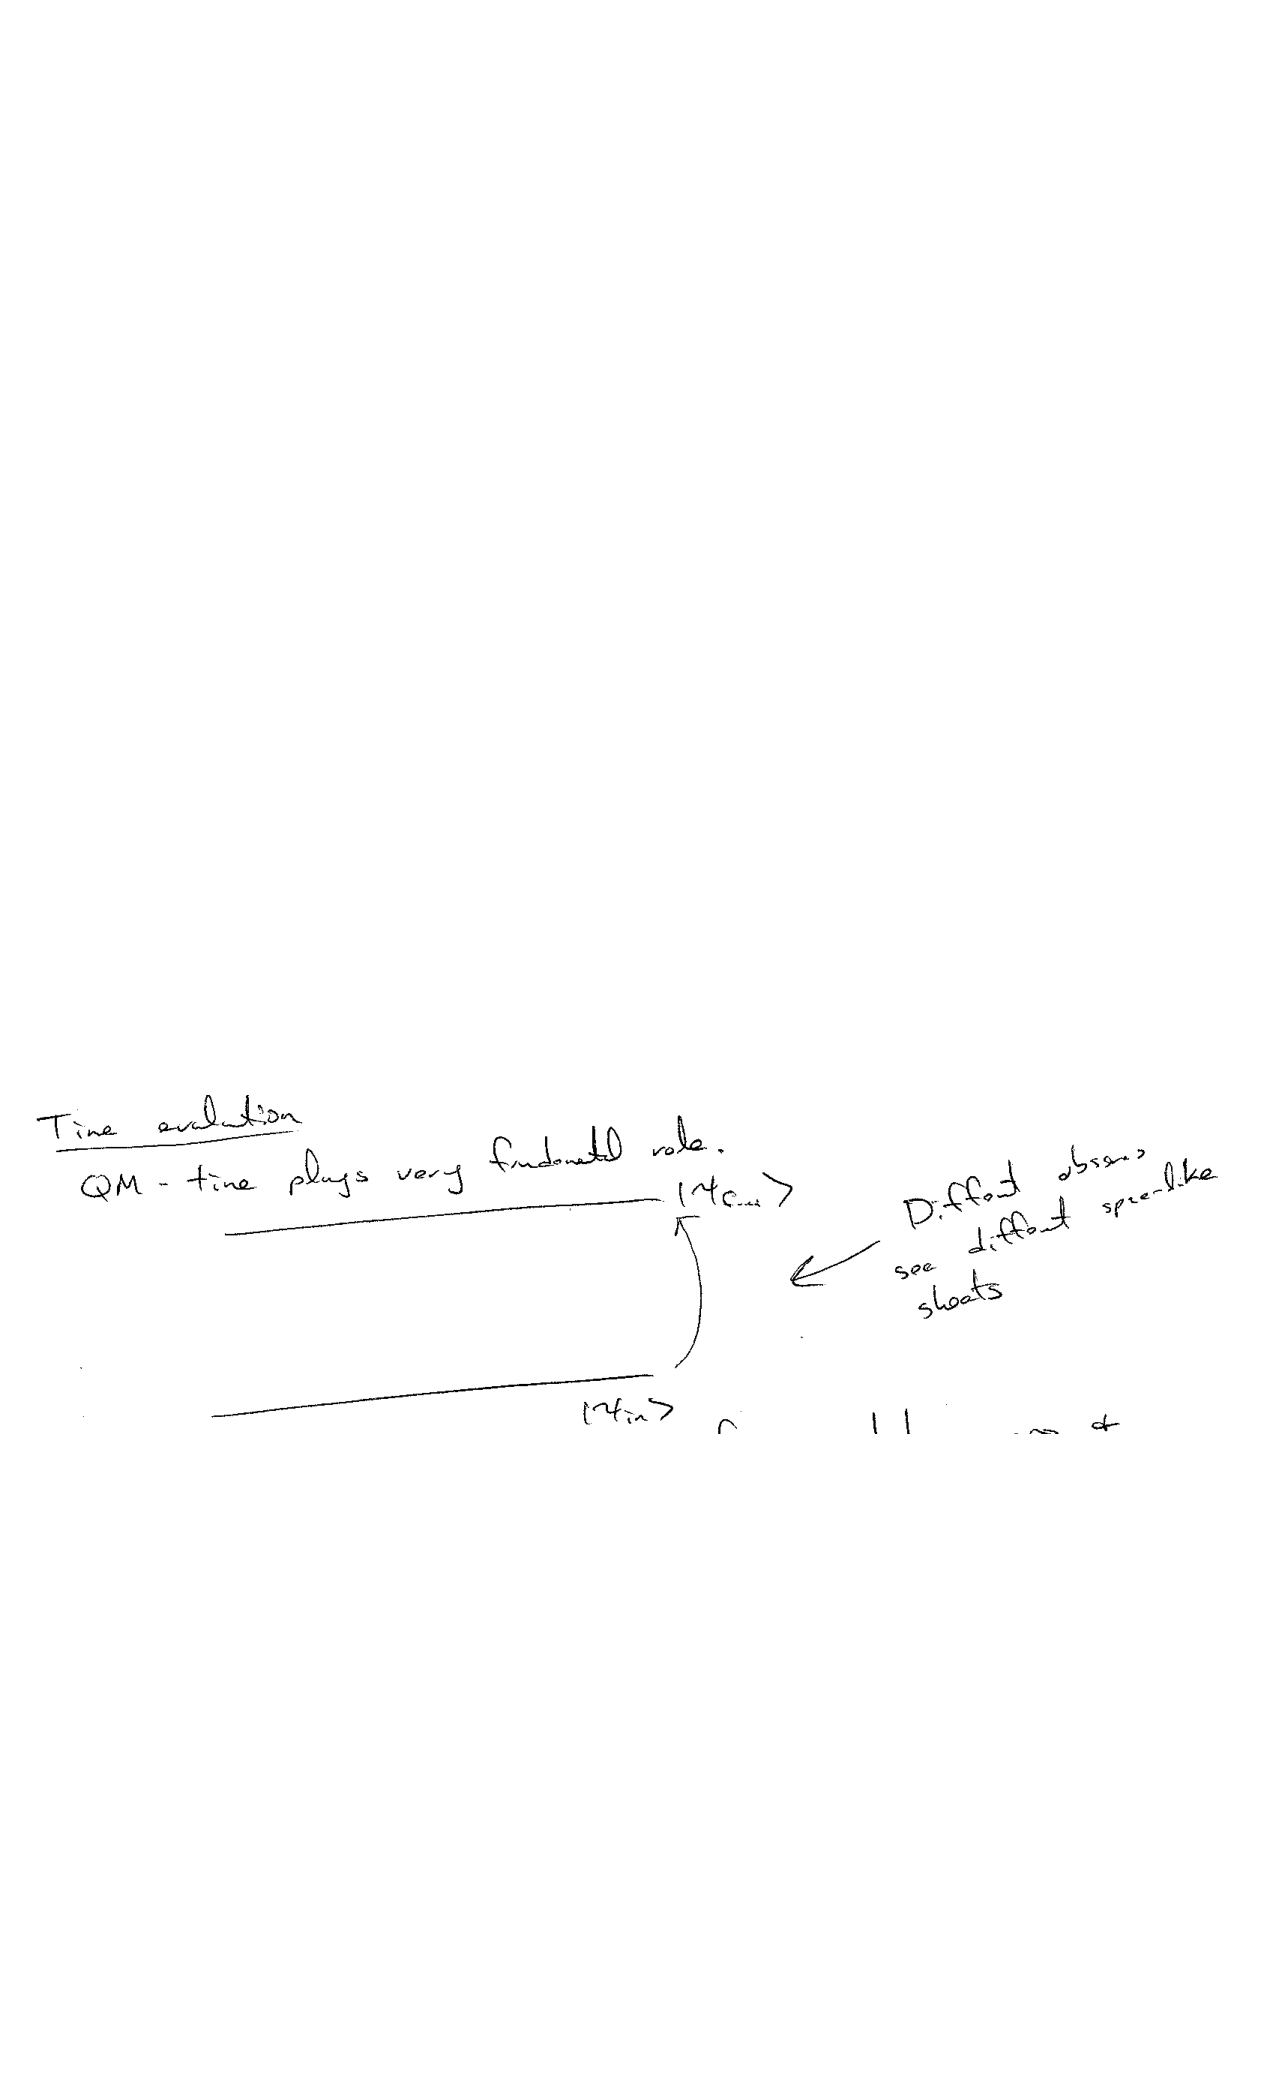
\includegraphics[width=0.9\textwidth]{./TimeEvolution.pdf}
\end{figure}

Only have a hope of Lorentz invariance if we start at -$\infty$ and go to +$\infty$.

Throw particles in from $\infty$ let them scatter \& go back out to $\infty$.

\underline{Define S-Matrix}

\be
\underbrace{\ket{p_1 \sigma_1,...p_n\sigma_n}}_{t=-\infty} \rightarrow \underbrace{\mathcal{S} \ket{p_1\sigma_1,...p_n\sigma_n}}_{t=+\infty}
\ee

$\mathcal{S}$ might be (at least a hope) Lorentz Invariant.


\noindent\rule{\textwidth}{1pt}

Big Picture:
The plan is to Figure out what $\mathcal{S}$ is in a tottaly generic theory, then see what it would take to make it Lorentz Invariant. 

Sure doesnt look like ti will be L.I. 
$\mathcal{S}$ is the only object that you could even have a hope to make L.I.

We will see that for \underline{very special} choices of the interaction it will barely be possible for it to be Lorentz Invariant. 
These choices force on us anti-particle and the connection between spin and statistics. 

\noindent\rule{\textwidth}{1pt}

Something annoying that we should get rid of right away. 
Free evolution, just evolves w/phase. Totally irrelevant part.


Standard way of removing the free evolution \underline{``Interaction Representation''}.

\be
H = H_\textrm{free} + H_\textrm{Int}
\ee


\be
i \frac{d \ket{\psi}}{d t} = \left(H_\textrm{free} + H_\textrm{Int} \right) \ket{\psi} 
\ee

\underline{For $H_\textrm{Int}$ = 0}

\be
\ket{\psi} = e^{-i H_f t} \ket{\psi_{in}}
\ee

Now, we dont have a free theory, but if the interaction is small going to be pretty close to evolving like this. 


\begin{equation}\label{eq:def}
\ket{\psi} = e^{-i H_f t} \underbrace{\ket{\psi_{I}}}_{\textrm{definition}}
\end{equation}

If $H_\textrm{Int} = 0, \ket{\psi_\textrm{Int}}$ doesnt evolve at all.
Bc there is $H_\textrm{Int}$, $\ket{\psi_\textrm{Int}}$ will evolve. 

\bea
i \frac{d }{d t} \ket{\psi} &=& H_\textrm{f} \ket{\psi} + e^{-i H_f t} i \frac{d }{d t} \ket{\psi_I} \\
&=& (H_f + H_\textrm{int}) e^{-i H_f t} \ket{\psi_I}
\eea

Note: first line from derivitive of~\ref{eq:def}, the second from the Schrodinger Equation.

The RHSs imply, 

\be
i \frac{d }{d t} \ket{\psi_I} =  \underbrace{e^{-i H_f t} H_\textrm{Int} e^{-i H_f t}}_{\textrm{Interaction Hamiltonian in the interaction representation}}  \ket{\psi_I} 
\ee


So, 

\be
i \frac{d }{d t} \ket{\psi_I} =  H_I  \ket{\psi_I} 
\ee
where $H_I$ can be time dependent. 

\underline{Lets formally sovle this} 

Just intergrating gives,

\be
\ket{\psi_I (t_2)} = \ket{\psi_I (t_1)} - i \int_{t_1}^{t_2} dt H_I \ket{\psi_I(t)}
\ee

Now we can keep iterating, 

\be
 = \ket{\psi_I (t_1)} - i \int_{t_1}^{t_2} dt H_I(t) \left( \ket{\psi_I (t_1)} - i \int_{t_1}^{t} dt' H_I(t') \ket{\psi_I(t')}\right)
\ee

or

\be
 = \ket{\psi_I (t_1)} - i \int_{t_1}^{t_2} dt H_I \ket{\psi_I (t_1)}  +  (-i)^2 \int_{t_1}^{t_2} dt \int_{t_1}^{t} dt' H_I(t)H_I(t')\ket{\psi_I(t')}
\ee

Pattern is clear,  can keep going...

\bea
\ket{\psi_I (t_2)} = [ &1& + (-i) \int_{t_1}^{t_2} dt H_I(t) \\
    &+& (-i)^2 \int_{t_1}^{t_2} dt \int_{t_1}^{t} dt' H_I(t)H_I(t') \\
    &+&  (-i)^3 \int_{t_1}^{t_2} dt \int_{t_1}^{t} dt' \int_{t}^{t'} dt'' H_I(t) H_I(t') H_I(t''') \\
    &+& ...  ] \ket{\psi_I (t_1)}
\eea

If $H_I$ is small this is giving us some nice perturbation theory. 

}
\end{document}


